\section{Application to AO Primitives}\label{Section:Application}

This section organizes the applications around three elimination patterns. The goal is to highlight the solving methodology first and to use concrete AO primitives as representative case studies. We focus on solving strategies rather than on new algebraic models for AO primitives, reusing the best-known models from the literature and reevaluating them through the Dixon-resultant viewpoint.

\begin{remark}
Although much of the preceding discussion is developed under genericity assumptions, the structural bounds remain applicable to non-generic polynomial systems arising in AO primitives. Estimates relying on heuristic assumptions remain conditional. These bounds may be loose for structured instances, but still provide useful complexity estimates for algebraic analysis.
\end{remark}

\subsection{Method 1: Direct elimination}\label{subsec:method1}
Method~1 applies the Dixon resultant directly to a square polynomial system. Starting from $n$ equations in $n$ variables, we eliminate $n-1$ variables, solve the resulting elimination polynomial in the remaining parameter, and then back-substitute recursively. The whole algebraic burden is concentrated in one structured determinant, so the complexity analysis reduces to the matrix-size and determinant models from Section~\ref{Section: Estimate}. This is the classical Dixon solving workflow of~\cite{cryptoeprint:2005/312,Albrecht2008}, instantiated here with the bounds of Section~\ref{Section: Complexity} and the implementation of Section~\ref{Section: Improvements}.

This method is best suited to Type~I (low-degree) primitives, whose CICO systems admit a dense but uniformly low-degree algebraic description, so that the first elimination dominates and the later back-substitution phases operate on lower-dimensional systems; we take \poseidon as the representative example.

\paragraph{Application to \poseidon.}
We consider the CICO-3 problems of \poseidon~\cite{DBLP:conf/uss/0001KR0S21} and \poseidonnew~\cite{DBLP:conf/africacrypt/GrassiKS23} in sponge mode, using the input/output and internal-subspace models from~\cite{DBLP:journals/tosc/GrassiKR25}; the precise models are summarized in Appendix~\ref{appendix:poseidon} (see Figure~\ref{fig:poseidon} for an overview of the permutation). For the pure I/O model, direct Dixon elimination matches the natural square-system viewpoint. For the mixed-degree subspace models, the Hessenberg bound from Section~\ref{Section: Complexity} becomes essential because the polynomial degrees are no longer uniform.
Figure~\ref{fig:poseidon_complexity} compares the resulting complexities for $t=8$, $c=d=3$, $\alpha=3$ across different numbers of partial rounds.

\begin{figure}[h]
\centering
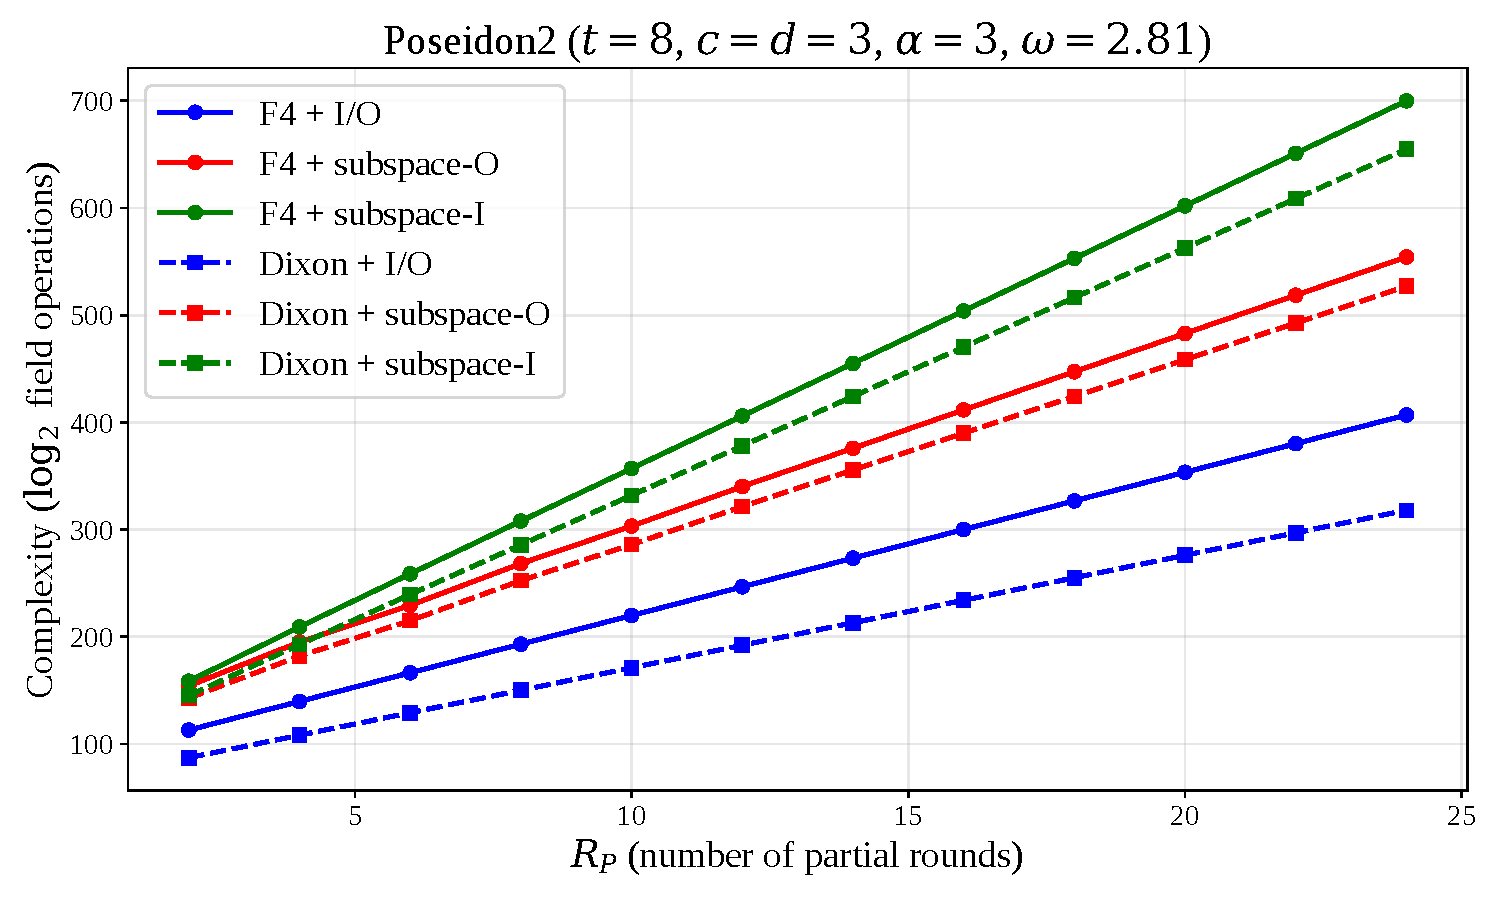
\includegraphics[width=0.95\textwidth]{poseidon_complexity.pdf}
\caption{Complexity comparison for \poseidon and \poseidonnew, with the model parameters $t=8$, $c=d=3$, $\alpha=3$ of~\cite{DBLP:journals/tosc/GrassiKR25}. Here $\omega = 2.81$ for all curves.}
\label{fig:poseidon_complexity}
\end{figure}

Table~\ref{tab:poseidon-timing} reports small-instance timings. Full-round systems behave close to generic dense systems, while partial-round systems are much more structured, so both the Dixon matrix size and the Gr\"obner-basis degree of regularity fall well below their generic upper bounds. Since the size of this drop depends on the specific subspace model, the generic bound should be read as an upper-bound template rather than as a tight prediction of the best attack. A finer analysis of these structural effects is left for future work.

\begin{table}[h]
\centering
\caption{Timing comparison for \poseidon instances ($t=6, c=1, d=3$, I/O modeling, bypass one round) over $\mathbb{F}_p$, $p = 2^{62}+169$. $T$ and $E$ denote theoretical and experimental values; complexities (Comp.) are in $\log_2$ field operations. Here $\omega = 2.81$. For odd $R_F$, one additional full round is added at the beginning. Both the Comp. and the timed implementation use the HNF determinant model.}
\label{tab:poseidon-timing}
\small
\setlength{\tabcolsep}{3.5pt}
\renewcommand{\arraystretch}{1.2}
\begin{tabular}{lcccccccccc}
\toprule
& \multicolumn{5}{c}{\textbf{Gr\"obner Basis}} & \multicolumn{5}{c}{\textbf{Dixon Resultant}} \\
\cmidrule(lr){2-6} \cmidrule(lr){7-11}
\textbf{Configuration} & \multicolumn{2}{c}{$d_{\text{reg}}$} & \multicolumn{2}{c}{Comp.} & Time & \multicolumn{2}{c}{$D(\mathcal{F})$} & \multicolumn{2}{c}{Comp.} & Time \\
\cmidrule(lr){2-3} \cmidrule(lr){4-5} \cmidrule(lr){7-8} \cmidrule(lr){9-10}
& T & E & T & E & (s) & T & E & T & E & (s) \\
\midrule
$R_F=3, R_P=0, \alpha=3$      & 25  & 25 & 32.8 & 32.8 & 2.2      & 117  & 108  & 24.1 & 23.7 & 0.3    \\
$R_F=3, R_P=0, \alpha=5$      & 73  & 71 & 45.2 & 44.9 & 94295    & 925  & 875  & 33.9 & 33.7 & 1477   \\
$R_F=4, R_P=0, \alpha=3$      & 79  & 79 & 46.2 & 46.2 & 188189   & 1080 & 1053 & 34.7 & 34.6 & 1772   \\
\midrule
$R_F=2, R_P=1, \alpha=3$ & 25  & 11 & 32.8 & 23.9 & 0.02     & 117   & 36   & 24.1 & 19.3 & 0.006  \\
$R_F=2, R_P=1, \alpha=5$ & 73  & 27 & 45.2 & 33.7 & 14.3     & 925  & 175  & 33.9 & 27.2 & 2.1    \\
$R_F=3, R_P=1, \alpha=3$ & 79  & 31 & 46.2 & 35.3 & 178      & 1080 & 891  & 34.7 & 33.9 & 695   \\
$R_F=2, R_P=2, \alpha=3$ & 79  & 24 & 46.2 & 32.4 & 0.4      & 1080  & 297  & 34.7 & 29.4 & 11.9   \\
\bottomrule
\end{tabular}
\end{table}

\subsection{Method 2: Iterative elimination}\label{subsec:method2}
Throughout this section calligraphic letters denote blocks: $\mathcal{F},\mathcal{P},\mathcal{R}$ are blocks of polynomials, $\mathcal{X},\mathcal{Z}$ are blocks of variables, and $|\mathcal{X}|$ is the number of variables in the block $\mathcal{X}$.

Method~2 is designed for ladder-structured systems and generalizes iterative two-polynomial elimination to local multipolynomial subsystems. It can be viewed as a generalization of the resultant-based approach of Yang et al.~\cite{DBLP:conf/asiacrypt/YangZYLT24} to multipolynomial Dixon elimination, and as an AO-oriented specialization of hybrid Dixon-matrix construction from~\cite{DengQiTangDuan2022}. We write such a system as
\begin{equation}
\mathcal{S}: \quad \mathcal{F}_1(\mathcal{X}_0,\mathcal{X}_1),\ \mathcal{F}_2(\mathcal{X}_1,\mathcal{X}_2),\ \ldots,\ \mathcal{F}_n(\mathcal{X}_{n-1},\mathcal{X}_n),
\label{eq:iterative_chain}
\end{equation}
with $|\mathcal{F}_1|=|\mathcal{X}_0|+1$ and $|\mathcal{F}_i|=|\mathcal{X}_{i-1}|$ for $2\le i\le n$. Eliminating successively,
\begin{equation}
R_1 = \mathrm{Res}_{\mathcal{X}_0}(\mathcal{F}_1),\;
R_2 = \mathrm{Res}_{\mathcal{X}_1}(R_1,\mathcal{F}_2),\;\ldots,\;
R_n = \mathrm{Res}_{\mathcal{X}_{n-1}}(R_{n-1},\mathcal{F}_n),
\label{eq:iterative_resultants}
\end{equation}
yields a univariate eliminant if $|\mathcal{X}_n|=1$, or a smaller system otherwise.

Assume each block $\mathcal{F}_j$ has common degree $d_j$. By B\'ezout, the ideal-theoretic eliminant produced at step $i$ satisfies
\begin{equation}
\deg(R_i)\le \prod_{j=1}^{i} d_j^{|\mathcal{F}_j|}.
\label{eq:iterative_degree_bound}
\end{equation}
The last step produces $R_n$ from $R_{n-1}$ and $\mathcal{F}_n$, by eliminating the variables in $\mathcal{X}_{n-1}$. Here $R_{n-1}$ has degree $D_{\mathrm{in}}:=\prod_{j=1}^{n-1} d_j^{|\mathcal{F}_j|}$ and each polynomial in $\mathcal{F}_n$ has degree $d_n$. Viewing this as Dixon elimination on one polynomial of degree $D_{\mathrm{in}}$ and $|\mathcal{F}_n|$ polynomials of degree $d_n$, the Unrestricted Bound~\eqref{eq:unrestricted_bound} gives matrix size at most $\binom{d_n|\mathcal{F}_n|-d_n+D_{\mathrm{in}}}{|\mathcal{F}_n|}$. The total $\mathcal{X}_n$-degree of the cancellation determinant is at most $D_{\mathrm{in}}+d_n|\mathcal{F}_n|$ (sum of the per-row degrees in the eliminated block), which in turn upper-bounds the entry-wise $\mathcal{X}_n$-degree of the resulting Step~4 polynomial matrix (Section~\ref{Section: Estimate} Step~4), so HNF gives
\begin{equation}
\widetilde{\mathcal{O}}\!\left((D_{\mathrm{in}}+d_n|\mathcal{F}_n|)\binom{d_n|\mathcal{F}_n|-d_n+D_{\mathrm{in}}}{|\mathcal{F}_n|}^{\omega}\right),
\label{eq:iterative_sequential_complexity}
\end{equation}
with the Hessenberg Bound~\eqref{eq:hessenberg_bound} available when the Unrestricted Bound is too coarse.

For meet-in-the-middle (MITM) instances, we split the chain into forward and backward parts meeting in a small middle block $\mathcal{Z}$:
\begin{equation}
\mathcal{F}_1(\mathcal{X}_0,\mathcal{X}_1),\ldots,\mathcal{F}_{n}(\mathcal{X}_{n-1},\mathcal{Z}),
\quad
\mathcal{F}'_1(\mathcal{Y}_0,\mathcal{Y}_1),\ldots,\mathcal{F}'_{m}(\mathcal{Y}_{m-1},\mathcal{Z}).
\label{eq:iterative_mitm_chain}
\end{equation}
Forward and backward eliminations give two middle-state relations of degrees
\[
D_{\mathrm{fwd}}=\prod_{j=1}^{n} d_j^{|\mathcal{F}_j|}, \qquad
D_{\mathrm{bwd}}=\prod_{j=1}^{m} {d'_j}^{|\mathcal{F}'_j|}.
\]
The final merge eliminates the middle block $\mathcal{Z}$ and, with $d_{\max}=\max(D_{\mathrm{fwd}},D_{\mathrm{bwd}})$, admits the coarse bound
\begin{equation}
\widetilde{\mathcal{O}}\!\left(d_{\max}^{\omega+1}\right).
\label{eq:mitm_complexity}
\end{equation}

The complexity of Method~2 is the maximum over all stages: every determinant of the forward and backward chains~\eqref{eq:iterative_sequential_complexity} and the final merge~\eqref{eq:mitm_complexity}. Root finding, back-substitution, and the verification of the candidate solutions in the original system---which also discards the spurious candidates possibly introduced by extraneous factors---are negligible in comparison.

This method is best suited to Type~II (equivalence-relation) primitives, whose ladder-structured CICO systems link successive states through local low-degree relations; we take \vision as the representative example.

\paragraph{Application to Vision.}
For \vision~\cite{DBLP:journals/tosc/AlyABDS20} with $s=2$, inverse layers make the full direct model unattractive, so we adopt a meet-in-the-middle (MITM) approach following the general framework of Liu et al.~\cite{DBLP:conf/asiacrypt/LiuMM24} and apply iterative Dixon elimination. The detailed model and equation distribution are in Appendix~\ref{appendix:vision} (the round function is recalled in Figure~\ref{fig:vision}); Figure~\ref{fig:vision_complexity_comparison} and Table~\ref{tab:vision_timing} summarize the outcome.

\begin{figure}[h]
\centering

\includegraphics[width=0.90\textwidth]{vision_complexity.pdf}
\caption{Complexity comparison for \vision ($\omega = 2$ for consistency with~\cite{DBLP:conf/asiacrypt/LiuMM24}).}
\label{fig:vision_complexity_comparison}
\end{figure}

For these parameters the final merge~\eqref{eq:mitm_complexity} dominates every forward and backward stage of the chain, so it alone determines the reported complexity; the stage-by-stage figures, together with a rank bound that keeps the intermediate rungs below the merge, are collected in Appendix~\ref{appendix:vision}. This is the structured regime where local elimination is preferable to direct elimination.

\begin{table}[h]
\centering
\caption{Experimental timing and complexity comparison for \vision ($s=2$). Complexities (Comp.) are in $\log_2$ field operations. $\omega = 2$ for consistency with~\cite{DBLP:conf/asiacrypt/LiuMM24}.}
\label{tab:vision_timing}
\setlength{\tabcolsep}{6pt}
\renewcommand{\arraystretch}{1.2}
\begin{tabular}{lcccccc}
\toprule
& \multicolumn{2}{c}{\textbf{2 rounds}} & \multicolumn{2}{c}{\textbf{3 rounds}} & \multicolumn{2}{c}{\textbf{4 rounds}} \\
\cmidrule(lr){2-3} \cmidrule(lr){4-5} \cmidrule(lr){6-7}
\textbf{Method} & Comp. & Time & Comp. & Time & Comp. & Time \\
\midrule
Gr\"obner basis~\cite{DBLP:conf/asiacrypt/LiuMM24} & 31.0 & 1.38s & 42.0 & 1d 4h & 53.0 & --- \\
Dixon resultant & 24.1 & 0.1s & 31.0 & 15m & 48.1 & 3d \\
\bottomrule
\end{tabular}
\end{table}

\subsection{Method 3: Ideal reduction and hybrid elimination}\label{subsec:method3}
Method~3 combines Dixon elimination with the reduction machinery developed for FreeLunch-style systems in~\cite{DBLP:conf/crypto/BariantBBHOR25}. We start from a triangular system
\begin{equation}
\mathcal{P}=\left\{
\begin{array}{l}
z_1^\alpha-f_1(x)=0,\\
z_2^\alpha-f_2(x,z_1)=0,\\
\vdots\\
z_n^\alpha-f_n(x,z_1,\ldots,z_{n-1})=0,\\
h(x,z_1,\ldots,z_n)=0,
\end{array}
\right.
\label{eq:freelunch_system}
\end{equation}
and use the reduction procedure \texttt{Reduce} of~\cite[Algorithm~1]{DBLP:conf/crypto/BariantBBHOR25}. For a polynomial $g$ of weighted degree $d_{\mathcal{P}_k}(g)$ in a single retained variable, the reduction cost is $\widetilde{O}(d_{\mathcal{P}_k}(g)(2\alpha-1)^n)$~\cite[Lemma~1]{DBLP:conf/crypto/BariantBBHOR25}, where $n$ is the number of levels in the triangular ideal $\mathcal{P}_k$. We take the reduced triangular system as input. If it must be constructed from an arithmetic circuit, its construction cost must be added separately~\cite[Proposition~4]{DBLP:conf/crypto/BariantBBHOR25}. For CICO-1 and a system that is a FreeLunch Gr\"obner basis, the optimized two-polynomial strategy of~\cite[Corollary~3]{DBLP:conf/crypto/BariantBBHOR25} applies directly and gives
\begin{equation}
\widetilde{O}\!\left(d_{\mathcal{I}}\alpha^2\left(\frac{2\alpha-1}{\alpha}\right)^{n+2}\right).
\label{eq:two_poly_complexity_main}
\end{equation}
For general CICO-$k$, we retain $|\mathcal{X}|=k$ input variables and build $k$ relations $R_1(\mathcal{X}),\ldots,R_k(\mathcal{X})$ in three phases.

\emph{(P1) Reduction.} Each output constraint $h_j$ is replaced by its normal form modulo the triangular ideal, using~\cite[Algorithm~1]{DBLP:conf/crypto/BariantBBHOR25}. Since the polynomials manipulated here are $k$-variate in $\mathcal{X}$, the coefficient-count factor of~\cite[Lemma~1]{DBLP:conf/crypto/BariantBBHOR25} is replaced by the dense coefficient count $B_k(e):=\binom{e+k}{k}$ of a $k$-variate polynomial of degree $e$, which is $\Theta(e^k)$ for fixed $k$. Reduction never increases the weighted degree, so with $\bar{D}:=\max_j d_{\mathcal{P}_k}(h_j)$ this phase costs
\begin{equation}
	T_{\text{red}} = \widetilde{O}\!\left(k\,B_k(\bar{D})\,(2\alpha-1)^n\right).
	\label{eq:reduction_cost}
\end{equation}

\emph{(P2) Successive elimination.} Reduction only lowers the exponents $\deg_{z_i}$ below $\alpha$; it does not by itself produce an element of $\mathbb{K}[\mathcal{X}]$. For each constraint, set $h_{j,n}=\operatorname{NF}_{\mathcal{P}_n}(h_j)$ and compute, for $i=n,\ldots,1$, $h_{j,i-1}=\operatorname{NF}_{\mathcal{P}_{i-1}}(\operatorname{Res}_{z_i}(h_{j,i},z_i^\alpha-f_i))$. Here $\mathcal{P}_i$ contains the first $i$ triangular equations and $R_j=h_{j,0}\in\mathbb{K}[\mathcal{X}]$. By~\cite[Lemma~2]{DBLP:conf/crypto/BariantBBHOR25} the stage with $i$ triangular levels remaining costs $\widetilde{O}(D_i(2\alpha-1)^{i+2})$ for a single retained variable, where $D_i \le \alpha^{\,n-i}\bar{D}$ bounds the weighted degree before eliminating $z_i$ at that stage~\cite[Lemma~3]{DBLP:conf/crypto/BariantBBHOR25}; here the factor $D_i$ is again replaced by $B_k(D_i)$. Summing over all stages and all $k$ constraints,
\begin{equation}
	T_{\text{elim}} = \widetilde{O}\!\left(k\sum_{i=1}^{n} B_k(D_i)\,(2\alpha-1)^{i+2}\right).
	\label{eq:successive_elim_cost}
\end{equation}
For fixed $\alpha$ and $k=1$, the geometric sum gives the bound of~\cite[Proposition~7]{DBLP:conf/crypto/BariantBBHOR25}, dominated by the first stage $i=n$. For fixed $k\ge 2$, since $B_k(D_i)=\Theta(D_i^{k})$ and $\alpha^{k}>2\alpha-1$, the sum is instead dominated by the last stage $i=1$. Note also that~\eqref{eq:reduction_cost} is always dominated by the term $i=n$ of~\eqref{eq:successive_elim_cost}.

\emph{(P3) Final elimination.} Let $d_{\mathcal{R}} := \max_j \deg(R_j)\le \alpha^{\,n}\bar{D}$. Assuming that $\langle R_1,\ldots,R_k\rangle$ is zero-dimensional and the Dixon projection conditions hold, the final step eliminates $k-1$ variables from these $k$ relations by mixed-degree Dixon elimination:
\begin{equation}
	T_{\text{final}} = \widetilde{O}\!\left(\max\left\{T_{1}^{\mathrm{best}}(\mathcal{R}),\,T_3(\mathcal{R}),\,k\,d_{\mathcal{R}}\,D(\mathcal{R})^{\omega}\right\}\right),
	\label{eq:hybrid_final_complexity}
\end{equation}
where $T_{1}^{\mathrm{best}}$ and $T_3$ are the construction and rank-extraction costs of Section~\ref{Section: Estimate}, and $D(\mathcal{R})$ is bounded by Corollary~\ref{cor:three_bounds}(3), which specializes to $C_k^{(d_{\mathcal{R}})}$ when all the $R_j$ have the same degree.

The total symbolic hybrid cost is, up to a constant factor, the maximum of~\eqref{eq:reduction_cost}--\eqref{eq:hybrid_final_complexity}; in particular the reduction and elimination phases are not absorbed into the final Dixon cost in general. By contrast, direct elimination on the unreduced system of $n+k$ equations gives
\begin{equation}
	\widetilde{O}\!\left(\max\left\{T_{1}^{\mathrm{best}}(\mathcal{P}_k),\,T_3(\mathcal{P}_k),\,\Bigl(\sum_i d_i\Bigr)D(\mathcal{P}_k)^{\omega}\right\}\right),
	\label{eq:hybrid_direct_complexity}
\end{equation}
again with $D(\mathcal{P}_k)$ from Corollary~\ref{cor:three_bounds}(3), since the constraints $h_j$ do not have the same degree as the triangular equations; the last term becomes $(n+k)\alpha (C_{n+k}^{(\alpha)})^{\omega}$ when all equations have degree $\alpha$. The comparison between the two routes determines whether the reduction phase is worthwhile.


This method is an improved attack on Type~II (equivalence-relation) primitives, refining Method~2 by interleaving Dixon elimination with ideal reduction; we take \xhash as the representative example.

\begin{remark}
	For the special case of CICO-1, the two-polynomial iterative-resultant route of~\cite{DBLP:conf/crypto/BariantBBHOR25} already gives~\eqref{eq:two_poly_complexity_main}, and Dixon does not change the picture. In concurrent and independent work, Bak et al.~\cite{DBLP:journals/iacr/BakBHN26} develop a related CICO-2 framework, introducing improvements to variable elimination and the final bivariate resultant, with substantial theoretical and practical gains. Although Method~3 does not currently offer a concrete advantage for $k\ge 3$, it provides a more flexible framework for further elimination strategies.
\end{remark}


\paragraph{Application to \xhash.}
We focus on \xhash~\cite{DBLP:journals/iacr/AshurKM23}; the permutation (Figure~\ref{fig:xhash12}) and the triangular model we use are recalled in Appendix~\ref{appendix:xhash}. Figure~\ref{fig:xhash_complexity} compares the direct Dixon method, the hybrid reduction-based strategy, and the corresponding generic Gr\"obner-basis estimate for each $k=1,2,3,4$. The hybrid method is excellent for CICO-1 and retains a small margin for CICO-2. For CICO-3 and CICO-4, however, the intermediate degrees make it worse than the direct elimination method.

\begin{figure}[t]
  \centering
  \begin{minipage}[t]{0.48\textwidth}
    \centering
    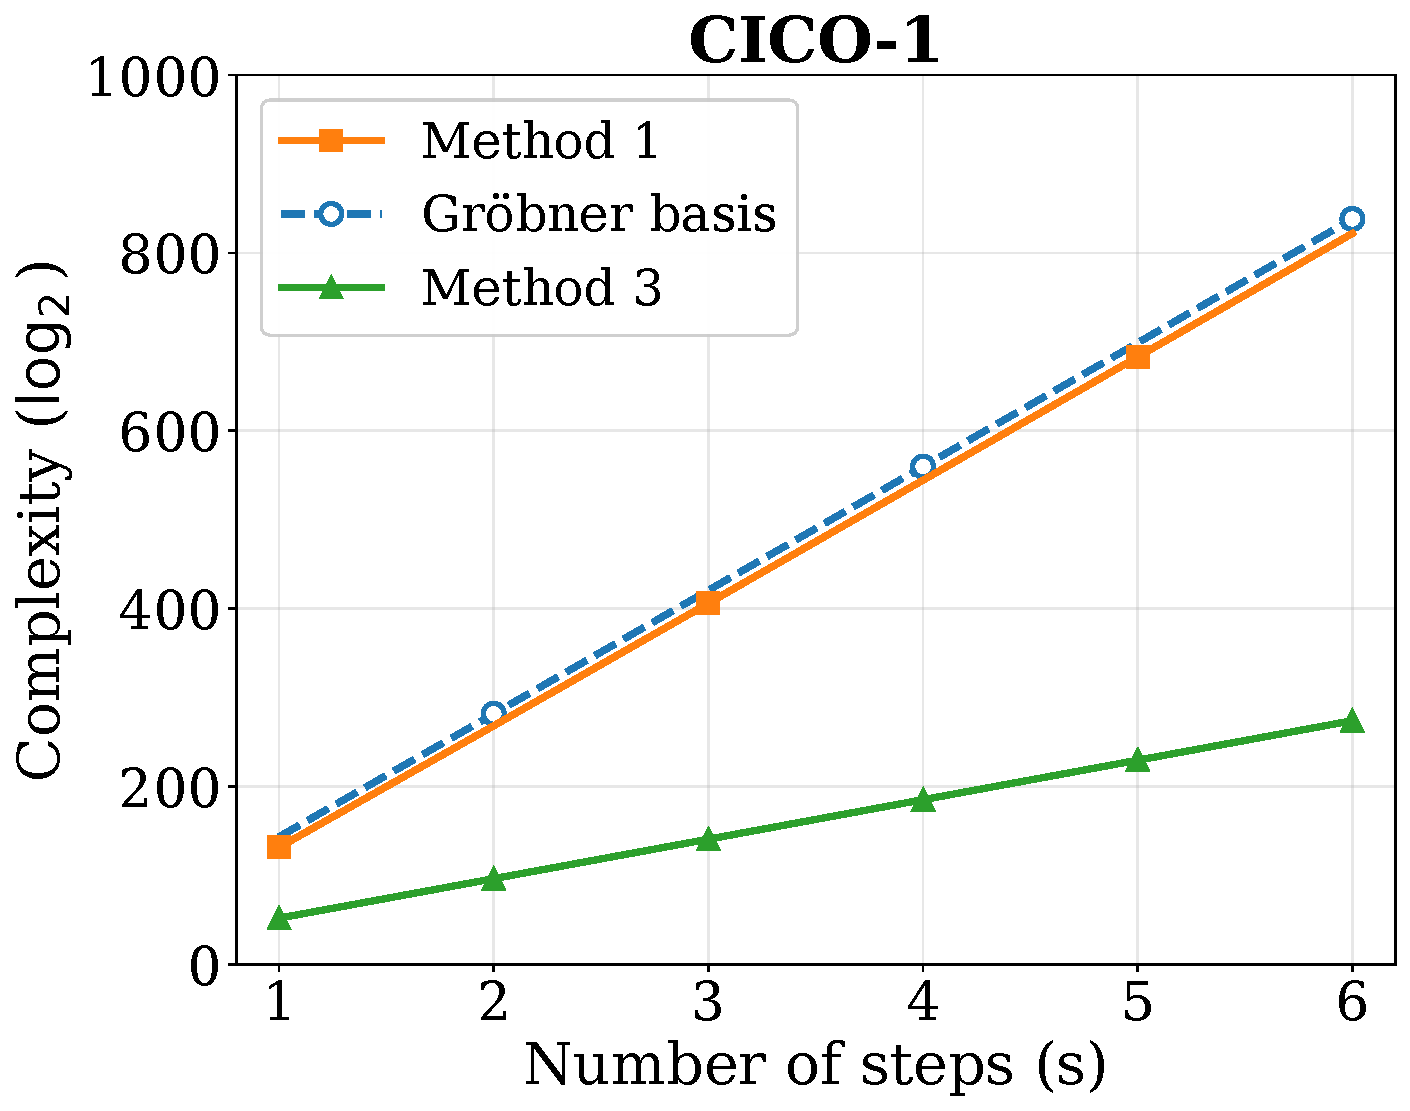
\includegraphics[width=\linewidth]{figure5_cico1.pdf}
  \end{minipage}\hfill
  \begin{minipage}[t]{0.48\textwidth}
    \centering
    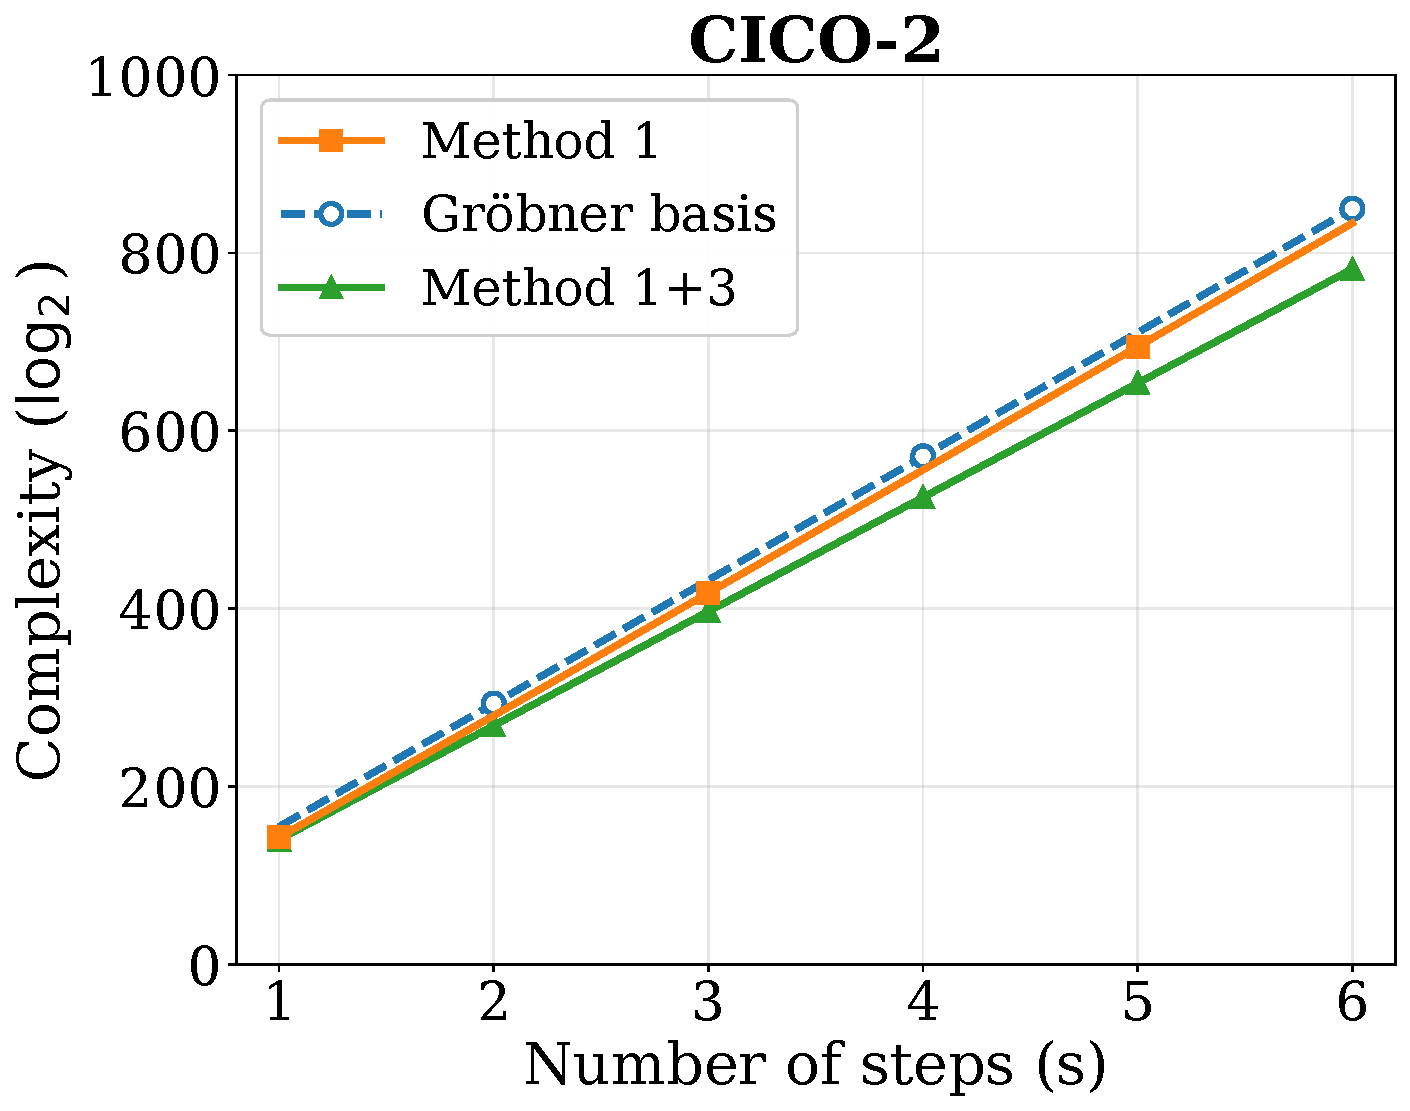
\includegraphics[width=\linewidth]{figure5_cico2.pdf}
  \end{minipage}\\[2pt]
  \begin{minipage}[t]{0.48\textwidth}
    \centering
    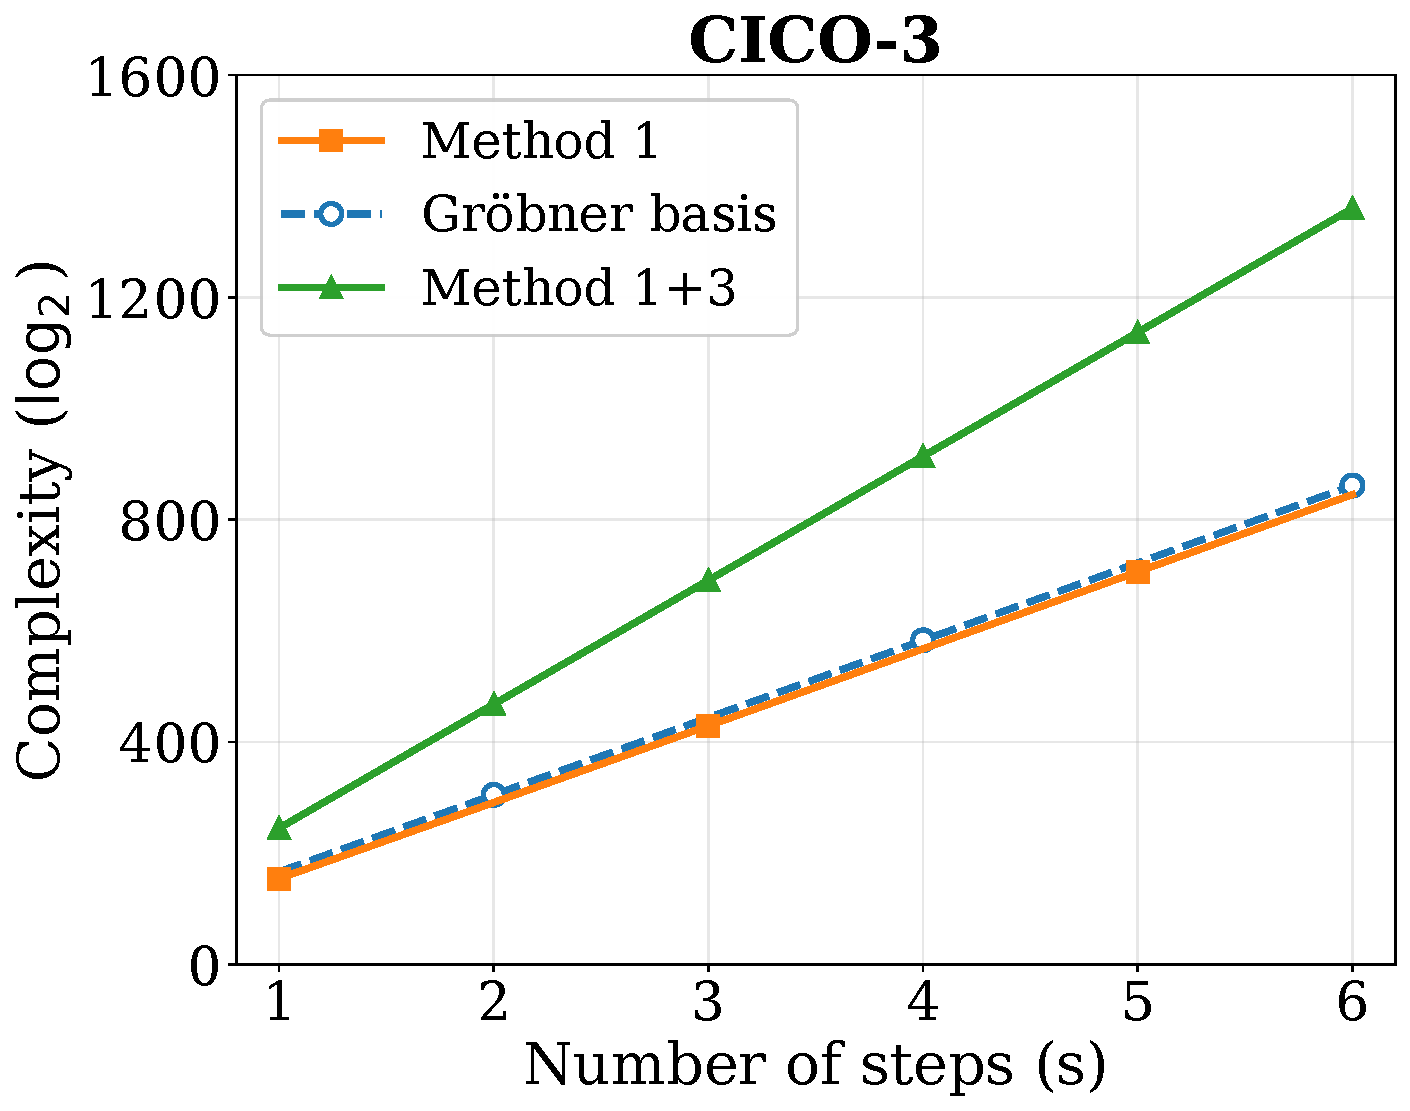
\includegraphics[width=\linewidth]{figure5_cico3.pdf}
  \end{minipage}\hfill
  \begin{minipage}[t]{0.48\textwidth}
    \centering
    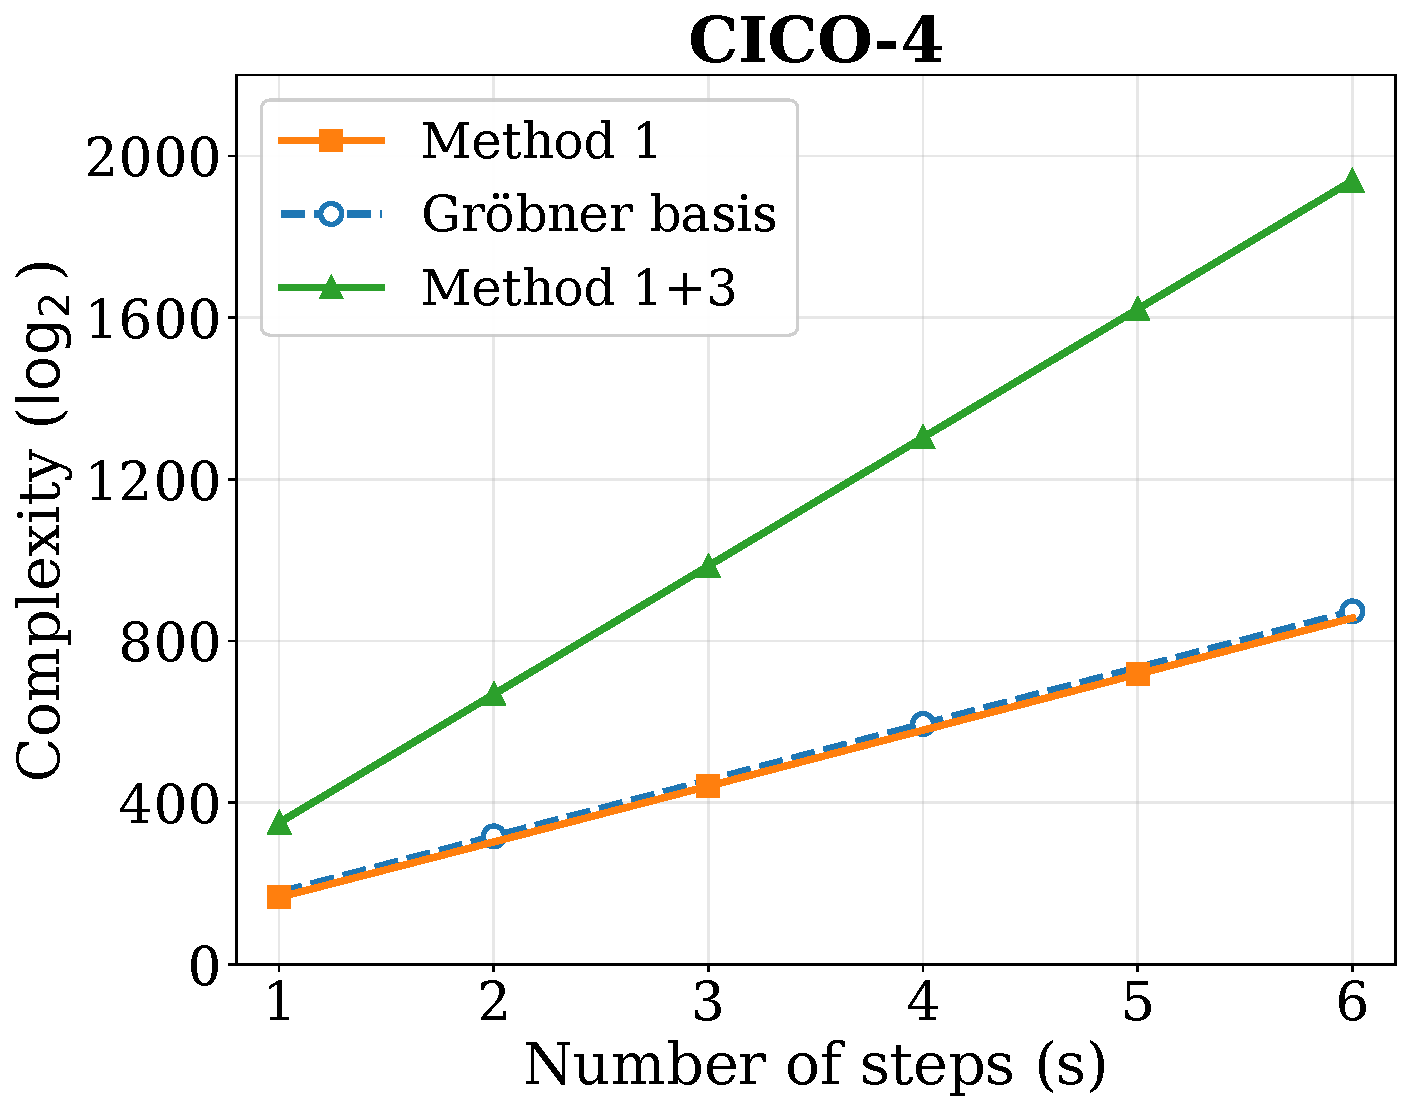
\includegraphics[width=\linewidth]{figure5_cico4.pdf}
  \end{minipage}
  \caption{Symbolic complexity comparison for \xhash,
    $\alpha=7$ and $\omega=2.81$, in $\log_2$ field operations.
    The CICO-1 Method~3 curve uses~\eqref{eq:two_poly_complexity_main}; the hybrid Method~1+3 for $k\ge2$
    includes reduction, successive elimination and final Dixon elimination.
    Each GB curve uses $\binom{m+d_{\mathrm{reg}}}{m}^{\omega}$,
    where $m=12s+k$ and $d_{\mathrm{reg}}=m(\alpha-1)+1$.}
  \label{fig:xhash_complexity}
\end{figure}

Table~\ref{tab:xhash_experimental} compares symbolic complexity estimates with recorded elimination times for small \texttt{XHash} polynomial systems. The special structure of these instances and implementation details can lead to discrepancies between generic complexity bounds and measured running times. A refined complexity analysis accounting for this structure is left for future work.

\begin{table}[!htbp]
\centering
\caption{Elimination times and symbolic complexity estimates for small \texttt{XHash} polynomial systems. The tuples specify $(\alpha,\mathrm{State},\mathrm{step})$: the exponent, state width, and number of steps. Comp. denotes $\log_2$ field operations with $\omega=2.81$.}
\label{tab:xhash_experimental}
\begin{tabular}{l|cc|cc|cc}
\toprule
 & \multicolumn{2}{c|}{CICO-1 $(3,3,5)$} & \multicolumn{2}{c|}{CICO-1 $(7,3,5)$} & \multicolumn{2}{c}{CICO-2 $(3,4,3)$} \\
\cmidrule{2-7}
Method & Comp. & Time & Comp. & Time & Comp. & Time \\
\midrule
Gr\"obner basis & 48.8 & 1.5s & 74.7 & - & 41.4 & 59.7s \\
Method 1 & 42.6 & 5.12s & 64.4 & - & 35.1 & 4.5s \\
Method 1+3 & 18.6 & 0.04s & 29.6 & 200.4s & 31.2 & 413.2s \\
\bottomrule
\end{tabular}
\end{table}
